\section{Deployment and Usage}
\label{sec:deployment}

A \ac{glsp} editor can be deployed and used in production in various ways. \ac{glsp} provides platform integrations for the Eclipse Desktop IDE, Eclipse Theia, \ac{vscode}, and as a standalone web application. Each integration brings different integration possibilities, deployment, and usage options for the editor. \cite{glsp-doc} The main considerations for the deployment and usage are:
  \begin{itemize}
    \item The user should need as few dependencies as possible. Dependencies are a browser runtime, an \acs{ide} to install, or an extension to install.
    \item The app should be easy to access. Possible barriers are the creation of an account or the installation of dependencies.
    \item Using a self-hosted server or a cloud service. With a self-hosted server, the user has full access of local files to open and edit. With a cloud service, the user has to upload and download files to the server.
  \end{itemize}
  
  To use \ac{glsp} as a standalone web application, a dependency injection container with the custom \ac{glsp} client is added to a TypeScript browser application. Like that the editor of a certain file as a data source can be displayed. When the app is hosted, no other dependency than a browser runtime is needed to use the standalone diagram editor. \cite{glsp-client-repo} This option provides the most flexibility, as it can be used in any web application, but also requires the most effort to implement, when developing a complete editor. All features, like file management, window management, or other features a \acs{ide} brings, need to be implemented by the developer. \cite{glsp-client-repo} For our use case, the standalone web application is not an option, as these additional features are needed. 

  The other \ac{glsp} integrations are \acs{ide} integrations and therefore provide many features out of the box. For the Eclipse \acs{ide} integration, Eclipse has to be installed, and the \ac{glsp} plugin has to be added to the Eclipse installation. The plugin can be installed from the Eclipse Marketplace or manually by downloading the plugin jar file. \cite{eclipse-doc} The \ac{vscode} integration also provides this option. The \acs{ide} can be installed and the \ac{glsp} editor can be added as an extension. The extension can be installed from the Marketplace or manually using a \textit{.vsix} file. \cite{vscode-doc} The \ac{glsp} \ac{vscode} integration can provide a \textit{.vsix} file. \cite{glsp-repo} \ac{vscode} is the most used \acs{ide}. 73.6\% of developers use \ac{vscode} due to the survey of \citeauthor{stackoverflow2024survey} In \citeyear{stackoverflow2024survey} \cite{stackoverflow2024survey}. An advantage to Eclipse is that \ac{vscode} provides a browser version, which brings the same capabilites as the desktop \acs{ide}. \cite{vscode-doc} So this integration provides the advantage that no \acs{ide} has to be installed to be able to use Henshin Web. The user can open \ac{vscode}, add the extension, and directly open a metamodel, rule, or instance model file and start editing. 

  The Eclipse Theia \acs{ide} is not as widely popular as \ac{vscode} \cite{stackoverflow2024survey}, but its focus is not to provide a ready \acs{ide} but to provide tools to create custom \acsp{ide}. The Eclipse Theia project is part of the Eclipse Foundation and is used as a basis to create your own \acsp{ide} based on web technologies. \cite{theia-doc} They provide the Theia IDE that acts as a template editor and can be downloaded and used on all common operating systems or used in as a web editor in the browser. Due to the focus on providing a framework to build custom \acsp{ide}, Theia provides more options to use extensions and plugins to extend the functionality. You can see the options and their architectural integration into Theia in figure \ref{fig:theia-extensions}.
  \begin{itemize}
    \item \textbf{\ac{vscode} extensions} Theia provides the \ac{vscode} extension \acs{api}, so that existing \ac{vscode} extensions can be used in Theia. They only interact with the \acs{api} and therefore can be installed at runtime.
    \item \textbf{Theia plugins} are working like \ac{vscode} extensions. They interact with the Theia plugin \acs{api} and can also access the \ac{vscode} extension \acs{api}. They can access some Theia specific features, that \ac{vscode} extensions cannot access, like directly contributing to the frontend. They can also be installed at runtime, or be pre-installed at compile time.
    \item \textbf{Headless plugins} are also working like \ac{vscode} extensions. They can also be installed at runtime and can access custom extended Theia backend services.
    \item \textbf{Theia extensions} are the core architecture parts of Theia. Theia is fully built using Theia extensions in a modular way. The template Theia \acs{ide} contains Theia extensions, including the core. Custom Theia extensions can be developed and added to Theia with full access to all Theia functionality via dependency injection. They need to be installed at compile time. \cite{theia-doc}
  \end{itemize}

  The \ac{glsp} Theia integration is creating a Theia extension, that is packed into a custom Theia \acs{ide}. It is also possible to use the \ac{glsp} \ac{vscode} integration that provides a \ac{vscode} extension, that can also be added to a Theia \acs{ide} at runtime. \cite{glsp-repo} The option to use the diagram editor in the browser makes the \ac{glsp} Eclipse integration not interesting for Hensin Web. \ac{vscode} has the advantage of popularity and simplicity to use the editor without any registration or installation. Eclipse Theia has the advantage of modularity and further extensibility. Further features can be added in the future to provide a web-based environment for \ac{mde}. Theia also provides different ways to deploy a Theia \acs{ide}.   These considerations show that the Theia integration is the best option for deploying the Henshin Web editor. Theia combines the advantages of browser-based access, modularity, and extensibility.

  \begin{figure}[h]
    \centering
    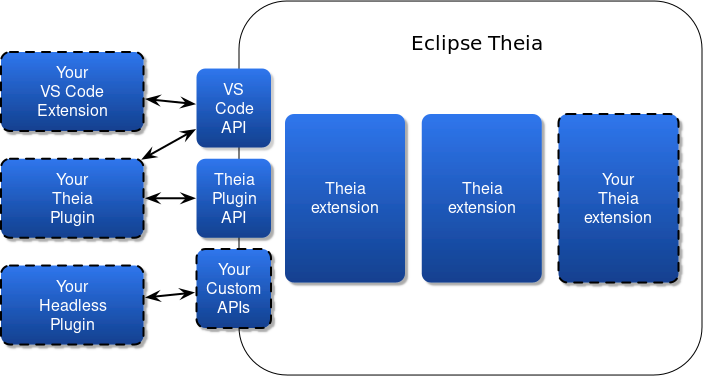
\includegraphics[width=0.7\textwidth]{theia-extension}
    \caption{Theia high level extensions and plugins architecture. Image obtained from \cite{theia-doc}}
    \label{fig:theia-extensions}
  \end{figure}

  There are different options to provide a \ac{glsp} Theia application. The Theia editor, consisting of the TypeScript client and the Java server, can be hosted in the cloud and accessed via a web browser. The Eclipse Foundation provides the Theia Cloud project \cite{theia-cloud-doc} to deploy Theia based products on Kubernetes clusters \cite{kubernetes}. Theia Cloud introduces three custom Kubernetes resource types. \textit{App Definitions} contain all necessary information about the Theia based product. \textit{Workspaces} define persistent storage solutions, where metamodel, rule, or instance model files can be stored for each user. \textit{Sessions} are acting as a runtime representaions. Theia Cloud includes components like a landing page, authentication, authorization, a cloud monitor, and a cloud operator, that deploys sessions and manages workspaces. You can see the different components and their interactions in figure \ref{fig:theia-cloud-components}. The service provides two preconfigured configurations for quickly trying out Theia Cloud on a cluster. \cite{theia-cloud-doc}

  \begin{figure}[h]
    \centering
    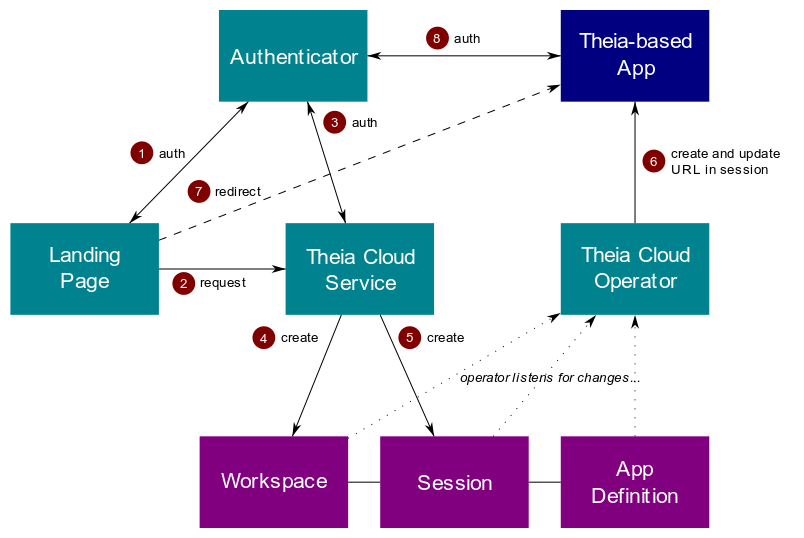
\includegraphics[width=0.7\textwidth]{theia-cloud-components.png}
    \caption{Interaction between Theia Cloud components. Image obtained from \cite{theia-cloud-doc}}
    \label{fig:theia-cloud-components}
  \end{figure}

  Because of the limited file access of the browser, the user has to upload and download all files to the server to use them. To be able to access the local file system of the user directly, the server needs to be hosted locally. For that, \ac{glsp} Theia application can be hosted in a Docker container. \cite{docker} The Docker container can contain the Java server and the TypeScript client, that are started together. The user can then access the editor via a web browser. On a machine with a Docker environment, this solution can be started locally in an easy way and has the access to the file system. The Docker container can also be used to deploy the application on a server so that it can be accessed by multiple users. The single Docker container solution doesn't provide as much scalability as using a cluster with Theia Cloud.

  The \ac{glsp} Theia application can also be used as a desktop application. Theia uses Electron \cite{electron-repo} to bundle the application into a desktop application, that can be installed via an installer. This approach also provides access to the local file system, since the electron application works like a self-hosted web application, and therefore the \ac{glsp} Java server is started locally. All in all, the \ac{glsp} Theia integration provides all different options to use the Henshin Web editor. Further clients can always be added later if needed.